% ============================================================================
%  第 17 章  几何 Langlands 中的边界条件
% ============================================================================
\chapter{几何 Langlands 中的边界条件}\label{ch:17}

\begin{flushright}
\small 第 36 讲；2021 年 8 月 24 日
\end{flushright}

具体地，我们将讨论几何 Langlands 中的边界条件在数论中的应用。

\begin{keytakeaways}
本章说明如何用几何 Langlands 中的边界条件统一处理 $L$-函数与周期。基本想法是：
$n$ 维规范场论的边界条件大致等同于带 $G$-对称的 $(n-1)$ 维理论；对四维 $\mathcal N=4$
超杨--Mills 理论，边界条件给出三维理论，其局部算子构成 $E_3$-代数，取相对谱便得到对偶群的
哈密顿空间。B-侧的边界条件（以哈密顿 $G^{\vee}$-空间 $M^{\vee}$ 为靶的 Rozansky--Witten 理论）
组织 Galois 表示的 $L$-函数：局部 $L$-因子是 Frobenius 在 $\operatorname{Sym}^{\bullet}V=\cO(M^{\vee})$
上的迹，整体 $L$-函数则是 $L$-可观测层的因子化同调（沿曲线取迹）。A-侧的边界条件
（球簇 $X$ 的余切丛 $T^*X$ 等哈密顿 $G$-空间）组织自守形式的周期，Plancherel 测度在几何上范畴化为
$M^{\vee}$。两者通过猜想 $|\mathcal{P}_X(\varphi)|^2=L(\rho,M^{\vee})$ 相联系。核心工具包括：相对谱、
因子化同调、几何 Satake、球簇、Iwasawa--Tate 理论以及 Hecke 代数与 $\Rep(G^{\vee})$ 的等价。
\end{keytakeaways}

\section{边界条件概述}

\begin{sectionkey}
本节给出全章的总图景：$n$ 维规范场论的边界条件是带 $G$-对称的 $(n-1)$ 维理论；对四维
$\mathcal N=4$ 超杨--Mills，A/B 扭转给出两类边界条件，而电磁对偶把 $G$ 的边界条件与
$G^{\vee}$ 的边界条件对应起来。由此，A-侧的哈密顿 $G$-空间与 B-侧的哈密顿 $G^{\vee}$-空间应当互相匹配。
\end{sectionkey}

粗略的想法是：$n$ 维规范场论（规范群为 $G$）的边界条件，大致应该是带 $G$-对称的
$(n-1)$ 维理论。首先我们举一些例子，作为真正关心的问题的热身。

\begin{srcex}{114}
若 $G$ 是紧 Lie 群，则存在一个二维 QFT，即拓扑杨--Mills 理论 $\mathrm{YM}^{top}_G$。
其边界条件是一维理论，现在带 $G$-对称，故边界条件的范畴是 $\Rep(G)$。
\end{srcex}

\begin{srcex}{115}
二维 A-型规范场论也被物理学家称为群 $G$ 在 A-扭转下的 $\mathcal N=(2,2)$ 超杨--Mills 理论。
我们如下给出该理论的边界条件。设 $G\curvearrowright X$。边界理论将是某种量子力学；
但代替 $X$ 上的普通量子力学，我们可以通过把 de Rham 复形 $H^{\bullet}_{dR}(X)$ 作为态空间，
在 $X$ 上做超对称量子力学。由于 $G\curvearrowright X$，我们可以问 de Rham 复形获得何种对称性。
它确实有作用，但方式使得 $\mathfrak g=\mathrm{Lie}(G)$ 的作用被平凡化。这正是著名的
Cartan 同伦恒等式的内容。故经典地，你只看到连通分量群在作用；但更丰富的说法是，事实上得到作用
\begin{equation}\tag{17.1}\label{eq:17.1}
H_*(G)\curvearrowright H^*(X).
\end{equation}
这些可以称为 $G$ 的\term{局部常值表示}{locally constant representation}，
而不是上一个例子中那样的普通表示。
\end{srcex}

这与我们将在四维 A-模型中看到的情形非常相似。特别地，这个理论中的局部算子看起来像
\begin{equation}\tag{17.2}\label{eq:17.2}
H_*(G)\otimes H^*(BG).
\end{equation}

% [Tutor Note: 式 (17.1) 中的 $H_*(G)$ 作用是 Cartan 模型给出的：$G$ 在 de Rham 复形上的
%  作用可同伦平凡化，从而在 $H^*(X)$ 上只剩 $H_*(G)$（即 $G$ 的链复形/群同调）的作用；
%  这就是为什么作者称其为“局部常值表示”而不是普通表示。对连通紧群，$H_*(G)\cong H^*(\Omega G)$，
%  它与 $H^*(BG)$ 通过 Koszul 对偶相关联，于是 (17.2) 中 $H_*(G)\otimes H^*(BG)$ 正是
%  $G$-等变上同调在自由作用情形下的局部模型。注意不要把 $H_*(G)$ 与群环 $\C[G]$ 混淆。]

在几何 Langlands 中，我们研究这个物理规范场论的边界条件，它称为四维
$\mathcal N=4$ 超杨--Mills 理论（Gaiotto--Witten），是一个 $G$-规范理论。
一个边界条件（原文此处标注 cite）是某种带 $G$-对称的三维理论。因为我们讨论的是超对称的
体理论，所以也需要适当超对称的边界理论。在物理中，若取一个流形 $M$，它不仅具有 Riemann 度量
（如 SUSY QM 所需），也不仅具有 Kähler 结构，而具有\term{超 Kähler}{hyperkähler}结构，
那么这恰好就是构造到 $M$ 的三维 $\sigma$-模型所需的条件。这最终是一个 $\mathcal N=4$
超对称理论（即有 8 个超荷）。我们应把它看作\term{2-移位量子化}{2-shifted quantization}的版本：
我们构造的不再是向量空间（即一维场论），而是三维 QFT。由于有足够的超对称，我们可以用几种方式
使它拓扑化。一种是“Coulomb”/B-扭转，给出以 $M$ 为靶的 Rozansky--Witten TFT。
还有“Higgs”/A-扭转，即鲜为人知的三维 A-模型。我们不打算真正讨论 A-模型。
超 Kähler 流形有很多结构，但特别地它是全纯辛的。对 Rozansky--Witten 理论，我们只需要 $M$
是全纯辛的，即实际上不需要 Riemann 度量。

设有一个紧群 $G_c$ 通过超 Kähler 等距作用 $G_c\curvearrowright M$。（或者我们可以考虑复群
$G_{\C}$ 通过全纯辛对称性作用 $G_{\C}\curvearrowright M$。）由这些数据，我们得到这个四维
$\mathcal N=4$ 杨--Mills 理论的一个边界条件。确实，类型是匹配的：A-型版本给出四维 A-理论
$\mathcal A_G$ 的边界条件，B-型版本给出四维 B-理论 $\mathcal B_G$ 的边界条件。
这将是我们边界理论的来源。

Gaiotto 与 Witten 告诉我们：若你有电磁/S-对偶，那么它是把 $G$ 的 $\mathcal N=4$ SYM 与
$G^{\vee}$ 的 $\mathcal N=4$ SYM 等同起来的对称性。既然理论本身被等同，边界条件也被等同。
于是我们得到 $\mathcal A_G$ 的边界条件与 $\mathcal B_{G^{\vee}}$ 的边界条件之间的对应。
在 $\mathcal A_G$ 的边界条件中，可以考虑“几何的”那些，它们来自哈密顿 $G$-空间
$G\curvearrowright M$。于是我们可能希望它们与来自哈密顿 $G^{\vee}$-空间
$G^{\vee}\curvearrowright M^{\vee}$ 的 Rozansky--Witten 理论相匹配。我们甚至可以更贪心一些，
希望真正匹配 A-侧上为余切丛的那些：
\begin{equation}\tag{17.3}\label{eq:17.3}
G\curvearrowright X;\quad M=T^*X
\qquad\overset{?}{\longleftrightarrow}\qquad
G^{\vee}\curvearrowright X^{\vee};\quad M^{\vee}=T^*X^{\vee}.
\end{equation}

\section{相对谱}

\begin{sectionkey}
本节说明：给定四维 TFT 的边界理论 $\mathcal T$，它在每个配边上给出一个元素
$\mathcal T(N)\in\cZ(N)$；对 $S^2$ 取这个元素，得到线算子范畴中的 $E_3$-代数，
其谱给出对偶群上的哈密顿空间 $M^{\vee}\to\mathfrak g^{\vee*}/G^{\vee}$，即“相对谱”。
\end{sectionkey}

回忆上次的内容：我们可以做得更好一些——给定一个边界条件，实际上可以构造一个哈密顿
$G$-空间或 $G^{\vee}$-空间。这就是“相对谱”构造。

设 $\cZ$ 是四维 TFT，边界理论/条件为 $\mathcal T$。这给出什么样的代数结构？
我们可以把 $\mathcal T$ 想成从平凡理论到 $\cZ$ 的映射：
\begin{equation}\tag{17.4}\label{eq:17.4}
\mathcal T\in\Hom(1,\cZ).
\end{equation}
这意味着，对维数 $\le 3$ 的 $N$，可以看 $\cZ(N)$，并得到
\begin{equation}\tag{17.5}\label{eq:17.5}
\mathcal T(N)\in\Hom\bigl(1,\cZ(N)\bigr).
\end{equation}
我们确实可以把它理解为定义了一个元素
\begin{equation}\tag{17.6}\label{eq:17.6}
\mathcal T(N)\in\cZ(N).
\end{equation}

\begin{srcrem}{118}
有时我们可以把它想成一个泛函
\begin{equation}\tag{17.7}\label{eq:17.7}
\mathcal T(N)\in\Hom\bigl(\cZ(N),1\bigr),
\end{equation}
但若没有足够的对偶性，这两者可能并不完全相同。
\end{srcrem}

于是边界理论在理论赋予每个配边的对象中挑出一个元素，方式与所有结构相容。例如，从配边
$S^2\times I$ 得到线算子范畴中的一个特定对象 $\mathcal T(S^2)\in\cZ(S^2)$，其中区间的
一端标以 $\mathcal T$。它与 $\cZ(S^2)$ 上的所有结构相容，即它是线算子范畴中的一个
$E_3$-代数对象。

思考这幅图的另一种方式如下。要描述边界上的局部算子，像所有缺陷一样，我们看该奇点的链环。
链环实际上就是一个三维球，其边界为 $S^2$。这幅图与上面配边 $S^2\times I$ 之间的关系很简单：
从 $B^3$ 中去掉奇点得到 $B^3\setminus \mathrm{pt}\simeq I\times S^2$。
结论是 $\mathcal T(S^2)\in\cZ(S^2)$ 是边界 $\mathcal T$ 上局部算子的 $E_3$-代数的一个相对细化：
通过把球填回去，即与单位线算子配对，可以得到局部算子的普通 $E_3$-代数。

也可以看 $\mathcal T$ 上的线算子。当我们切除某些线的管状邻域时，得到 $\mathcal T$ 的线算子带有
$\cZ$ 的线算子的作用。对我们而言，即当 $\cZ=\mathcal B_{G^{\vee}}$ 时，线算子为
\begin{equation}\tag{17.8}\label{eq:17.8}
\mathcal B_{G^{\vee}}(S^2)=\QC\bigl(\mathfrak g^{\vee*}/G^{\vee}\bigr),
\end{equation}
这里省略了移位 2。现在若有一个边界条件 $\mathcal T$，则 $\mathcal T(S^2)$ 是
$\QC(\mathfrak g^{\vee*}/G^{\vee})$ 中的一个 $E_3$（分次 Poisson）代数。
于是取其谱，得到余伴随表示上的仿射簇
\begin{equation}\tag{17.9}\label{eq:17.9}
M^{\vee}/G^{\vee}\to\mathfrak g^{\vee*}/G^{\vee},
\end{equation}
它就是 $M^{\vee}$ 作为哈密顿 $G^{\vee}$-空间的矩映射。这就是所谓相对谱的含义：它生活在
$\mathfrak g^{\vee*}/G^{\vee}$ 之上。若只取 $\mathcal T(S^2)$ 的非相对谱，则只得到
\begin{equation}\tag{17.10}\label{eq:17.10}
\Spec\cO(M^{\vee})^{G^{\vee}}\simeq M^{\vee}/\!/G^{\vee},
\end{equation}
即所谓仿射 GIT 商。所以它只是一个仿射 Poisson 簇。但做相对版本时，我们从线算子得到真正的哈密顿
$G^{\vee}$-空间。或者，如果你愿意，给定这样的映射 $M^{\vee}/G^{\vee}\to\mathfrak g^{\vee*}/G^{\vee}$，
可以过渡到层范畴，而 $M^{\vee}$ 上的（$G^{\vee}$-等变）层通过拉回被
$\mathfrak g^{\vee*}/G^{\vee}$ 上的层作用：
\begin{equation}\tag{17.11}\label{eq:17.11}
\QC\bigl(\mathfrak g^{\vee*}/G^{\vee}\bigr)\curvearrowright\QC(M^{\vee})^{G^{\vee}}.
\end{equation}
即 $\mathcal T$ 的线算子被 $\mathcal B_{G^{\vee}}$ 的线算子作用。

注意，我们关于边界条件需要知道的只是它的局部算子，而由几何 Satake，这些对 A-理论与 B-理论
是相同的。故我们可以不在意是从 A-侧还是 B-侧的边界条件出发。

于是想法是：从理论 $\mathcal A_G$ 的边界条件（即哈密顿 $G$-空间）出发，然后从它构造某种谱，
即这个 $G^{\vee}$ 的哈密顿空间。（这与 Braverman--Finkelberg--Nakajima 的 Coulomb 分支构造
非常相似，只不过我们在四维而非三维。）然后我们可能希望这个新空间 $M^{\vee}$ 正是我们的空间
$M$ 的真正对偶，即这个构造实现了 $\mathcal A_G$ 的边界条件与 $\mathcal B_{G^{\vee}}$ 的
边界条件之间的对偶。

% [Tutor Note: “相对谱”一词的关键在于 (17.9) 中的映射是到 $\mathfrak g^{\vee*}/G^{\vee}$
%  而非到点：通常的 $\Spec$ 只给出 $\cO(M^{\vee})^{G^{\vee}}$，丢掉等变结构；
%  相对版本把 $\mathcal T(S^2)$ 看作 $\QC(\mathfrak g^{\vee*}/G^{\vee})$ 中的 $E_3$-代数，
%  其相对谱保留了矩映射与 $G^{\vee}$-作用。另外 (17.8) 中省略的“移位 2”是
%  $S^2$ 作为二维流形带来的 cohomological shift；在线算子范畴中它对应
%  $\QC(\mathfrak g^{\vee*}/G^{\vee})$ 的 2-移位辛结构。]

\section{$L$-函数（B-侧）}

\begin{sectionkey}
本节解释 B-侧边界条件与 $L$-函数的关系：局部 $L$-因子是 Frobenius 在
$\operatorname{Sym}^{\bullet}V$ 上的迹，整体 $L$-函数是其 Euler 积；把对称代数实现为
某个空间上的函数（或层），就能把 $L$-值写成配分函数/迹。
\end{sectionkey}

现在我们想在两侧解释边界条件，并把它们与数论中感兴趣的对象联系起来。也就是说，B-侧的边界条件
将与 $L$-函数相关，A-侧的边界条件将与周期相关。首先我们讨论如何解释 B-侧的边界条件，
以及它们与 $L$-函数的关系。

回忆我们之前已经稍微讨论过这一点，例如在第 13.4 节。基本机制如下。我们有一个向量空间 $V$
及其自同态 $F\circlearrowleft V$。$L$-函数的局部版本是特征多项式的“超”版本。通常的特征多项式可写成
\begin{equation}\tag{17.12}\label{eq:17.12}
\det(1-tF)=\operatorname{Tr}_{gr}(F,\wedge^{\bullet}V).
\end{equation}
类似地，
\begin{equation}\tag{17.13}\label{eq:17.13}
\frac{1}{\det(1-tF)}=\operatorname{Tr}_{gr}(F,\operatorname{Sym}^{\bullet}V).
\end{equation}
事实上我们应该同时考虑这两者：若 $V$ 是超向量空间（即有偶部与奇部），则外代数就是奇部的对称代数。
例如，若 $V^{\bullet}$ 是链复形（微分无关紧要，故可只把它想成分次向量空间），则可以结合这两个公式
定义类似的 $L$-因子：
\begin{align}
L(V,F,t)&=\prod\det\bigl((1-tF)|_{H^k(V)}\bigr)^{(-1)^{k+1}}\tag{17.14}\label{eq:17.14}\\
&=\prod\operatorname{Tr}_{gr}\bigl(F,\operatorname{Sym}H^k(V)\bigr)\tag{17.15}\label{eq:17.15}\\
&=\operatorname{Tr}_{gr}(F,\operatorname{Sym}^{\bullet}V).\tag{17.16}\label{eq:17.16}
\end{align}
这里我们从记号中省略了 $H^k(V)$ 上的一些宇称修正，而 $\operatorname{Sym}^{\bullet}$ 是分次对称代数。

所以我们应把 $L$-因子看作特征多项式的某种版本。与通常的特征多项式不同（后者是有限的），
$L$-因子一般不是有限公式。也就是说，若 $V$ 有偶部，我们会得到 $t$ 的幂级数。
关于 $L$-函数可能有两个主要问题：一是关于对 $t$ 的依赖的解析问题（例如 Riemann 假设），
但这里我们感兴趣的是 $L$-值：
\begin{equation}\tag{17.17}\label{eq:17.17}
L(V,F)=L(V,F,t=1).
\end{equation}
例如，若 $F=\operatorname{id}$，则 $L(V,F)=\dim(\operatorname{Sym}(V))$。对一般的 $F$ 有
$L(V,F)=\operatorname{Tr}\bigl(F|_{\operatorname{Sym}(V)}\bigr)$。由于 $\operatorname{Sym}(V)$
通常是无穷维的，这个数一般没有意义。要点是这个数需要某种重正化。一个要点是：这个 $\infty$
与量子场论中出现的 $\infty$ 是同一类：在 QFT 中你常常写下最终无穷的配分函数表达式，
于是需要某种正则化或重正化程序。在我们这里，$L$-值将字面地作为配分函数出现，
而实际上重正化的技术往往与物理中相同。

这算是函数域的记号，但我们也可以用更经典数论的记号来写这个 $L$-值，那里没有单个变量 $t$。
我们确实必须把 $t=q^{-s}$，其中 $q$ 是素数的幂（局部域情形中剩余域的阶）。
想法是 $t$ 是乘法变量，于是加法变量 $s$ 是 $t$ 的“对数”。但若有不同的素数，必须区别对待。
我们之前谈过一点，想法是数域有点像三维流形。它并不真的纤维化在圆周上：每个素数都有一个“圆周”，
而每个都有一个“长度”，大致是 $\log p$。例如你会看到如下表达式
\begin{equation}\tag{17.18}\label{eq:17.18}
\frac{1}{\det(1-p^{-s}F)},
\end{equation}
故 $p^{-s}$ 扮演 $t$ 的角色。由于我们考虑 $L$-函数在 $t=1$ 处的值，这对应 $s=0$。
改变求值点，例如从 $s=0$ 过渡到 $s=n\in\Z$，对应于改变向量空间 $V$ 的分次。特别地，
\begin{equation}\tag{17.19}\label{eq:17.19}
L\bigl(V,F,t=q^{-k/2}\bigr)=L(V,F,s=k/2)=L(V\langle k\rangle,F,s=0),
\end{equation}
其中 $V\langle k\rangle$ 表示 $F\circlearrowleft V\langle k\rangle$ 通过 $q^{-k/2}F$ 作用。
这对我们不太重要，只是说精确的求值点并不那么重要：$L$-函数在 $s\in\Z$ 处的值等同于另一个
$L$-函数在 $s=0$ 处的值。故我们将谈论 $F\circlearrowleft V$ 的 $L$-值。这又一次完全绕开了
$L$-函数在 $s$ 中的解析性质问题。

\begin{srcex}{116}
在数论中遇到的第一个 $L$-函数是 Riemann $\zeta$-函数：
\begin{equation}\tag{17.20}\label{eq:17.20}
\zeta(s)=\sum_{n=1}^{\infty}\frac{1}{n^s}.
\end{equation}
也可以通过 Euler 积来看它：
\begin{equation}\tag{17.21}\label{eq:17.21}
\zeta(s)=\prod_p\frac{1}{1-p^{-s}}.
\end{equation}
于是我们从所有 $p$ 的 $L$-因子出发，取乘积得到 $L$-函数。如果你愿意，此情形中的算子 $F$
就是恒等。即这个 $L$-因子是考虑带恒等算子作用的平凡一维向量空间时得到的。于是我们可能对
$L$-值感兴趣：
\begin{equation}\tag{17.22}\label{eq:17.22}
\zeta(0)=\sum 1=\#\mathbb{N}=-\frac{1}{2}.
\end{equation}
\end{srcex}

让我们把它放到所需的框架中。设 $G^{\vee}$ 是约化群，代替自同态，考虑某个元素
$F\in G^{\vee}$ 以及表示
\begin{equation}\tag{17.23}\label{eq:17.23}
V\colon G^{\vee}\to GL(V).
\end{equation}
然后想在这个框架中给出特征多项式的某种版本。对这个 $F$ 与 $V$，可以附着 $L$-因子
\begin{equation}\tag{17.24}\label{eq:17.24}
L(V\circlearrowleft F).
\end{equation}
特别地，若有一个 Galois 表示
\begin{equation}\tag{17.25}\label{eq:17.25}
\Gal(\overline{\Q}_p/\Q_p)\to G^{\vee},
\end{equation}
我们可以问这个表示是否非分歧，即它是否通过 Frobenius 分解：
\begin{equation}\tag{17.26}\label{eq:17.26}
\begin{array}{ccc}
\Gal(\overline{\Q}_p/\Q_p) & \xrightarrow{\qquad} & G^{\vee}\xrightarrow{\ V\ }GL(V)\\[2pt]
& \searrow & \nearrow\ \text{（虚线）}\\[2pt]
& \langle F\rangle &
\end{array}
\end{equation}
然后就可以对它附着 $L$-因子。

% [Tutor Note: (17.14)--(17.16) 中“$\det$ 的 $(-1)^{k+1}$ 次幂”容易出错：对 $k$ 为偶数
%  （偶上同调），指数为 $-1$，故取 $\det$ 的倒数；对 $k$ 为奇数，指数为 $+1$。
%  这正是超迹 $\operatorname{Tr}_{gr}=\operatorname{Tr}_{even}-\operatorname{Tr}_{odd}$
%  在对称/外代数上的体现。另 (17.22) 的 $\zeta(0)=\sum 1=\#\mathbb{N}=-1/2$ 是 $\zeta$ 的
%  解析延拓值（正则化），并非通常意义下发散级数的和；作者用它是为了强调 $L$-值需要重正化。]

这些就是局部因子，而我们可以如下为 Galois 表示定义整体 $L$-函数。设有表示
\begin{equation}\tag{17.27}\label{eq:17.27}
\Gal(F)\xrightarrow{\ \rho\ }G^{\vee}\xrightarrow{\ V\ }GL(V).
\end{equation}
则可以定义
\begin{equation}\tag{17.28}\label{eq:17.28}
L(\rho,V,s)=\prod_p L_p\bigl(V\circlearrowleft\rho(F_p)\bigr),
\end{equation}
其中 $F_p$ 是 $p$ 处的 Frobenius。先验地，在表示分歧的地方这并没有定义。
在除有限多个位之外的所有位，这个表示通过 Frobenius 分解，故我们可以只限制到它非分歧的位；
或者若 $p$ 分歧，仍可如下定义 $p$ 处的 $L$-因子。$p$ 处的 Frobenius 不再作用在 $V$ 上，
但它作用在惯性群的不变量上：
\begin{equation}\tag{17.29}\label{eq:17.29}
V^{Inertia}\circlearrowleft\rho(F_p).
\end{equation}
惯性群是核
\begin{equation}\tag{17.30}\label{eq:17.30}
Inertia\to\Gal(F_p)\to\langle F\rangle.
\end{equation}
这个 $L$-函数有点像作用在 $\bigotimes_p\operatorname{Sym}V$ 上的 Frobenius 算子的大张量积的迹，
但我们必须取惯性不变量：
\begin{equation}\tag{17.31}\label{eq:17.31}
L(\rho,V,s)=\operatorname{tr}\Bigl(\bigotimes_p F_p\circlearrowleft
\bigotimes_p\operatorname{Sym}V^{I_p}\Bigr).
\end{equation}
同样，正如 $\zeta$ 一样，它在 $s=0$ 处不收敛，但存在某个收敛区域；我们可以问能否解析延拓
并在 $s=0$ 处求值。

若 $C$ 是 $\F_q$ 上的曲线，则有 $C$ 的 Galois 群的非分歧部分：
\begin{equation}\tag{17.32}\label{eq:17.32}
\Gal^{unram}(C)=\pi_1^{arith}(C),
\end{equation}
它映到由 Frobenius 生成的 $\Z$ 的一个拷贝，其核是几何 $\pi_1$：
\begin{equation}\tag{17.33}\label{eq:17.33}
\pi_1^{geom}(C)\to\pi_1^{arith}(C)\to\langle F\rangle,
\end{equation}
其中
\begin{equation}\tag{17.34}\label{eq:17.34}
\pi_1^{geom}(C)=\pi_1\bigl(\overline C=C\times_{\F_q}\overline{\F}_q\bigr).
\end{equation}
于是图景是：若有一条有限域上的曲线，并把它想成纤维化在圆周上的三维流形，则我们有到圆周
$\pi_1$ 的映射，而核是纤维的 $\pi_1$。这个几何 $\pi_1$ 扮演上面惯性群的角色。
于是在此情形可以把 $L$-函数定义为单个 Frobenius 作用在 $\pi_1^{geom}$-不变量上的迹。

\subsection{整体函数域}

\begin{sectionkey}
本小节在函数域情形中把上一节的 $L$-函数几何化：固定局部系统
$\rho\in\Loc_{G^{\vee}}(C)$，则整体 $L$-值等于 Frobenius 在
$H^*(C,V_{\rho})$ 的对称代数上的迹；把对称代数实现为某个映射的函子（L-可观测层），
就把 $L$-函数变成几何对象上的函数。
\end{sectionkey}

现在我们对数论中的 $L$-函数稍有讨论，接下来要在函数域情形中更缓慢地把这些讲一遍。
我们想以更几何的方式解释这个 $L$-函数。

考虑曲线 $C/\F_q$，设 $V$ 是约化群 $G^{\vee}$ 的表示。我们要研究映入 $G^{\vee}$ 的 Galois 表示。
我们还将取 $V$ 是自对偶的，事实上是辛的。这与任意表示的 $L$-函数的一般理论相关：
若你对一般表示 $W$ 感兴趣，则 $T^*W=W\oplus W^*$ 将是辛的，于是
\begin{equation}\tag{17.35}\label{eq:17.35}
L(T^*W)=L(W)\cdot L(W^*).
\end{equation}
现在固定一个 Galois 表示。我们现在在几何中，故这是 $\pi_1$ 的表示，即固定某个局部系统
$\rho\in\Loc_{G^{\vee}}(C)$。回忆此语境中的局部系统是
\begin{equation}\tag{17.36}\label{eq:17.36}
\Loc_{G^{\vee}}(C)=\bigl\{\pi_1^{arith}\to G^{\vee}\bigr\}\big/G^{\vee}.
\end{equation}
这就是所谓\term{算术局部系统}{arithmetic local system}。在有限域上的曲线情形，它等同于
$C/\F_q$ 上被 Frobenius $F$ 固定的局部系统。注意我们假设处处非分歧。人们可以尝试在分歧情形
做其中许多事情，但那更难。

现在可以谈 $L$-值 $L(\rho,V)$。我们有 $\pi_1(C)\to G^{\vee}\circlearrowright V$，故可以取
\begin{align}
L(\rho,V)&=L(\rho,V,s=0)\tag{17.37}\label{eq:17.37}\\
&=L\bigl(V^{\pi_1^{geom}}\circlearrowleft F\bigr).\tag{17.38}\label{eq:17.38}
\end{align}
现在我们想更几何地解释它。在整个算术 $\pi_1$ 内部，有几何部分，它作用在 $V$ 上：
\begin{equation}\tag{17.39}\label{eq:17.39}
\rho\colon\pi_1^{geom}\to\End(V).
\end{equation}
换言之，$V$ 定义了一个向量空间的局部系统 $V_{\rho}$，它由 $\rho$ 作为 $G^{\vee}$-局部系统
与表示 $V$ 相伴而来。于是上面的向量空间实际上就是以这个局部系统为系数的上同调：
\begin{equation}\tag{17.40}\label{eq:17.40}
L(\rho,V)=L\bigl(H^*(C,V_{\rho})\circlearrowleft F\bigr).
\end{equation}
这就是我们的整体 $L$-函数。

我们可以用几种方式说这件事。我们在 $\Loc_{G^{\vee}}$ 上有一个万有层，由
\begin{equation}\tag{17.41}\label{eq:17.41}
\rho\mapsto H^*(C,V_{\rho})
\end{equation}
给出。即以万有局部系统的 $V$-扭为系数的 $C$ 的上同调。也就是说，我们有 $C\times\Loc_{G^{\vee}}$
上的层 $\{V_{\rho}\}$（在 $\Loc$ 方向拟凝聚，在 $C$ 方向局部常值（局部系统）），
然后可以沿映射
\begin{equation}\tag{17.42}\label{eq:17.42}
\begin{array}{c}
C\times\Loc_{G^{\vee}}\\[2pt]
\downarrow{\scriptstyle \pi}\\[2pt]
\Loc_{G^{\vee}}
\end{array}
\end{equation}
前推它。

于是我们有这个空间与 Frobenius 自同构：
\begin{equation}\tag{17.43}\label{eq:17.43}
\Loc_{G^{\vee}}(\overline C)\circlearrowleft F,
\end{equation}
其不动点是算术局部系统：
\begin{equation}\tag{17.44}\label{eq:17.44}
\Loc^{arith}_{G^{\vee}}=\Loc_{G^{\vee}}(C).
\end{equation}
在不动点 $\rho$ 处，
\begin{equation}\tag{17.45}\label{eq:17.45}
F\circlearrowleft fiber=H^*(C,V_{\rho}),
\end{equation}
而我们取迹得到 $L$。于是给定群的任一表示，我们得到算术局部系统空间
$\Loc^{arith}_{G^{\vee}}$ 上的函数 $\rho\mapsto L(\rho,V)$。

所以我们附着了 $\rho\mapsto\operatorname{Tr}\bigl(F\ \text{在}\ \operatorname{Sym}H^{\bullet}(C,V_{\rho})\ \text{上}\bigr)$。
我们想真正把这个对称代数当回事。特别地，它是交换环，我们想把
$\operatorname{Sym}H^{\bullet}(C,V_{\rho})$ 看作某个导出概形上的函数。要点是这个概形有很好的解释。
例如，若 $\rho$ 平凡，则有
\begin{equation}\tag{17.46}\label{eq:17.46}
\operatorname{Sym}H^{\bullet}(C,V)=\cO\bigl(\operatorname{Map}_{lc}(C,V)\bigr).
\end{equation}
对一般 $\rho$，我们有生活在 $C$ 上的 $V_{\rho}$，可以看局部常值截面：
\begin{equation}\tag{17.47}\label{eq:17.47}
\begin{array}{c}
V_{\rho}\\[2pt]
\downarrow\\[2pt]
C
\end{array}
\end{equation}
于是
\begin{equation}\tag{17.48}\label{eq:17.48}
\operatorname{Sym}H^*(C,V_{\rho})=\cO\bigl(\text{$V_{\rho}\to C$ 的局部常值截面}\bigr).
\end{equation}
现在以更统一的方式写这件事。某个时刻我们可能会在 $V$ 与 $V^*$ 之间马虎（例如
$\operatorname{Sym}V$ 与 $\operatorname{Sym}V^*$），但我们取 $V$ 是辛的，故它自对偶。
当对所有 $\rho$ 把这些组装起来时，得到空间
\begin{equation}\tag{17.49}\label{eq:17.49}
\begin{array}{ccc}
\Loc^{V}_{G^{\vee}} & = & \bigl\{\rho+\text{$V_{\rho}$ 的平坦截面}\bigr\}
=\operatorname{Map}_{lc}(C,V/G^{\vee})\\[2pt]
\downarrow & & \\[2pt]
\rho\in\Loc_{G^{\vee}} & = & \operatorname{Map}_{lc}(C,\mathrm{pt}/G^{\vee})
\end{array}
\end{equation}
现在定义
\begin{equation}\tag{17.50}\label{eq:17.50}
\cA_V\in\QC^{!}\bigl(\Loc_{G^{\vee}}\bigr),
\end{equation}
由
\begin{equation}\tag{17.51}\label{eq:17.51}
\cA_V:=\pi_*\cO
\end{equation}
给出。即它把
\begin{equation}\tag{17.52}\label{eq:17.52}
\rho\mapsto\cO(\text{$V_{\rho}$ 的局部常值截面})=\operatorname{Sym}H^{\bullet}(C,V_{\rho}).
\end{equation}
这一切的要点是：我们把这个对称代数纳入了几何故事。换言之，可以不写出对称代数而写出 $L$-函数：
\begin{equation}\tag{17.53}\label{eq:17.53}
L(V,\rho)=\operatorname{Tr}\bigl(F\ \text{在}\ \cA_V\ \text{于}\ \rho\ \text{处纤维上的作用}\bigr).
\end{equation}
这就是“$L$-可观测”层。它是交换代数的层。

\begin{srcrem}{119}
注意 $\Loc_{G^{\vee}}(C)$ 上的函数恰好是 $\mathcal B_{G^{\vee}}(C)$，其中我们把 $C$ 想成三维流形的
一个版本。事实上，我们刚刚看到它也来自几何对象上的层：
\begin{equation}\tag{17.54}\label{eq:17.54}
\cA_V\in\QC^{!}\bigl(\Loc_{G^{\vee}}\overline C\bigr)
=\mathcal B_{G^{\vee}}(\overline C).
\end{equation}
\end{srcrem}

对整个过程，我们其实不需要 $V$ 是向量空间。可以用某个簇 $M^{\vee}\circlearrowleft G^{\vee}$
替换 $V$。真正重要的是用哈密顿 $G^{\vee}$-空间替换辛表示 $V$。现在可以定义 $M^{\vee}$ 的
$L$-函数类比。我们有空间
\begin{equation}\tag{17.55}\label{eq:17.55}
\begin{array}{c}
\Loc^{M^{\vee}}_{G^{\vee}}=\operatorname{Map}_{lc}(C,M^{\vee}/G^{\vee})\\[2pt]
\downarrow{\scriptstyle \pi}\\[2pt]
\Loc_{G^{\vee}}
\end{array}
\end{equation}
然后可以把 $L$-可观测层定义为结构层的前推：
\begin{equation}\tag{17.56}\label{eq:17.56}
\cA_{M^{\vee}}=\pi_*\cO.
\end{equation}
于是可以在 $\rho$ 处的纤维上取 Frobenius 的迹：
\begin{equation}\tag{17.57}\label{eq:17.57}
\rho\in\bigl(\Loc_{G^{\vee}}\bigr)^{\mathrm{Fr}}=\Loc^{arith}_{G^{\vee}},
\end{equation}
即算术局部系统，便得到广义 $L$-函数。若 $\pi_1\to G^{\vee}\circlearrowright M^{\vee}$
有离散不动点，则得到切空间 $L$-函数之和。

\begin{srcrem}{120}
我们从整体故事出发，而辛结构起了什么作用一直不清楚。当我们把它与局部故事联系起来时，
这一点就会显现。
\end{srcrem}

\subsection{局部故事}

\begin{sectionkey}
本小节说明 Euler 积在 $\operatorname{Tr}(F)$ 解范畴化下是因子化同调的影子：局部 $L$-因子由
$\cO(M^{\vee})\in\Rep(G^{\vee})$ 给出，而其函子化/范畴化版本把局部数据放到
$\QC(\mathfrak g^{\vee*}/G^{\vee})$ 中；沿曲线取因子化同调便还原整体 $L$-函数。
\end{sectionkey}

在这个 $\operatorname{Tr}(F)$ 解范畴化之下，Euler 积是因子化同调的影子。

设 $G^{\vee}\circlearrowright V$（更一般地 $G^{\vee}\circlearrowright M^{\vee}$）。
则 $\cO(M^{\vee})$（或 $\operatorname{Sym}V^*$）是 $G^{\vee}$ 的表示。由这些可以定义局部 $L$-因子：
\begin{equation}\tag{17.58}\label{eq:17.58}
L^{local}(M^{\vee})=\bigl\{g\mapsto\operatorname{Tr}\bigl(g,\cO(M^{\vee})\bigr)\bigr\}.
\end{equation}
同样，这些函数会有很多极点。例如取恒等元素，我们要计算的是对称代数的维数。

但总有意义的一件事是范畴化版本。$\cO(M^{\vee})$ 是 $\Rep(G^{\vee})$ 中的交换代数。
若 $M^{\vee}$ 是哈密顿的，则有矩映射
\begin{equation}\tag{17.59}\label{eq:17.59}
M^{\vee}\xrightarrow{\ \mu\ }\mathfrak g^{\vee*}.
\end{equation}
于是可以前推，
\begin{equation}\tag{17.60}\label{eq:17.60}
\mu_*\cO_{M^{\vee}}=\int\QC\bigl(\mathfrak g^{\vee*}/G^{\vee}\bigr)
=\QC\bigl(\mathfrak g^{\vee*}\bigr)^{G^{\vee}}.
\end{equation}
所以我们是在取 $G^{\vee}$ 上的函数，并以与群作用相容的方式把它铺到余伴随表示上。

% [Tutor Note: (17.58) 中 $\operatorname{Tr}(g,\cO(M^{\vee}))$ 一般没有意义（$\cO(M^{\vee})$
%  无穷维，且 $g$ 的特征值连续），这正是作者说“有很多极点”的意思：它只是形式上的迹，
%  真正的对象是 (17.60) 中的 $\mu_*\cO_{M^{\vee}}$。另外 (17.60) 的等号应理解为
%  $G^{\vee}$-等变层的（导出）函子化版本，而不是逐点相等；右端的 $\QC(\mathfrak g^{\vee*})^{G^{\vee}}$
%  是 $G^{\vee}$-等变拟凝聚层，对应 $\mathfrak g^{\vee*}/G^{\vee}$ 上的 QC 层。]

现在要点是：$L$-函数的 Euler 积展开在这个范畴化世界中对应于因子化同调。这是一个关键想法，
但并没有真正写下来。它在 Gaitsgory--Lurie 的“Weil 关于 Tamagawa 数的猜想”中被提到。

回忆 Euler 积说 $L$-函数可以用局部 $L$-因子表达（原文此处标注 cite）：
\begin{align}
L(\rho,V)&=\prod_{x\in C}L_x(\rho,V)\tag{17.61}\label{eq:17.61}\\
&=\prod\operatorname{Tr}(\operatorname{Sym}V)\tag{17.62}\label{eq:17.62}\\
&=\operatorname{Tr}\Bigl(\bigotimes\operatorname{Sym}V\Bigr).\tag{17.63}\label{eq:17.63}
\end{align}
于是 $L$-函数是一个巨大张量积的迹。一般想法是：因子化同调也是某个巨大张量积的版本。
若 $R$ 是交换环，则按定义因子化同调接收来自
\begin{equation}\tag{17.64}\label{eq:17.64}
\int_C R\leftarrow\bigotimes_{x\in C}R
\end{equation}
的映射。事实上它是按如下关系取的商：每当你看到两个邻近的点，即两处各有一份 $R$，
就有一个映射 $R\otimes R\to R$。这在拓扑/Betti 情形最容易表述。在任意域上的曲线情形，
可以用 Ran 空间的概念来形式化。我们应把它想成张量积的某种改进版本：你在曲线的所有点上取这个
巨大张量积，然后按某些关系取商，使它变成合理的东西：
\begin{equation}\tag{17.65}\label{eq:17.65}
\int_C R=\cO\bigl(\operatorname{Map}_{lc}(C,\Spec(R))\bigr).
\end{equation}
于是若每个环都有 Frobenius 算子，我们可能想在这个无穷对称积上计算迹，但一般不收敛。
不过可以尝试与这个更好的对象上的 Frobenius 迹比较，得到被正则化的东西。

在我们的框架中，有这个局部范畴：
\begin{equation}\tag{17.66}\label{eq:17.66}
\QC\bigl(\mathfrak g^{\vee*}/G^{\vee}\bigr)=\mathcal B_{G^{\vee}}(S^2),
\end{equation}
然后可以尝试沿曲线计算它的因子化同调，结果是
\begin{align}
\int_C\QC\bigl(\mathfrak g^{\vee*}/G^{\vee}\bigr)
&=\QC\Bigl(\operatorname{Map}_{lc}\bigl(C,\mathfrak g^{\vee*}/G^{\vee}\bigr)\Bigr)\tag{17.67}\label{eq:17.67}\\
&=\QC\bigl(T^*[1]\Loc_{G^{\vee}}\bigr).\tag{17.68}\label{eq:17.68}
\end{align}
另一方面，我们有局部对象
\begin{equation}\tag{17.69}\label{eq:17.69}
\cO(M^{\vee}/G^{\vee})\in\QC\bigl(\mathfrak g^{\vee*}/G^{\vee}\bigr),
\end{equation}
它给出局部 $L$-因子。于是
\begin{equation}\tag{17.70}\label{eq:17.70}
\QC\bigl(T^*[1]\Loc_{G^{\vee}}\bigr)=\int_C\QC\bigl(\mathfrak g^{\vee*}/G^{\vee}\bigr),
\end{equation}
而在其中我们有
\begin{equation}\tag{17.71}\label{eq:17.71}
\QC\bigl(T^*[1]\Loc_{G^{\vee}}\bigr)\ni
\cO\Bigl(\Loc^{M^{\vee}}_{G^{\vee}}=\operatorname{Map}_{lc}(C,M^{\vee}/G^{\vee})\Bigr)
=\int_C\cO(M^{\vee}/G^{\vee}).
\end{equation}
于是有
\begin{equation}\tag{17.72}\label{eq:17.72}
\begin{array}{ccc}
\Loc^{M^{\vee}}_{G^{\vee}} & \xrightarrow{\ \mu\ } & T^*[1]\Loc_{G^{\vee}}
=\operatorname{Map}\bigl(C,\mathfrak g^{\vee*}/G^{\vee}\bigr)\\[2pt]
\downarrow & & \downarrow\\[2pt]
\Loc_{G^{\vee}} & = & \operatorname{Map}\bigl(C,\mathrm{pt}/G^{\vee}\bigr)
\end{array}
\end{equation}
于是从某种意义上说，因子化同调下降为与 $M^{\vee}$ 相伴的 $L$-函数的 Euler 积。

\subsection{小结}

\begin{sectionkey}
本小节总结 B-侧：Galois 表示的 $L$-函数是边界条件可观测量的 Frobenius 迹；局部数据是
$\cO(M^{\vee}/G^{\vee})$，整体可观测量是因子化同调 $\int_C\cO(M^{\vee})$，而几何量子化给出
携带其作用的 $L$-层。
\end{sectionkey}

总结一下：B-侧的边界条件/理论是组织 Galois 表示 $L$-函数的一种方式。
于是对线性表示 $G^{\vee}\circlearrowright W$，可以把它加倍得到辛向量空间
$V=W\oplus W^*$；更几何地，对 $G^{\vee}\circlearrowright X^{\vee}$，得到哈密顿 $G^{\vee}$-空间
\begin{equation}\tag{17.73}\label{eq:17.73}
T^*X^{\vee}=M^{\vee}\xrightarrow{\ \mu\ }\mathfrak g^{\vee*}.
\end{equation}
由此得到整体 $L$-函数：
\begin{equation}\tag{17.74}\label{eq:17.74}
\{L(\rho,V)\}\in\cO\bigl(\Loc_{G^{\vee}}(C)\bigr)=\mathcal B_{G^{\vee}}(C).
\end{equation}
另一方面，$L$-函数的局部数据是
\begin{equation}\tag{17.75}\label{eq:17.75}
\cO(M^{\vee}/G^{\vee})\in\operatorname{Alg}\Bigl(\QC\bigl(\mathfrak g^{\vee*}/G^{\vee}\bigr)\Bigr),
\end{equation}
即边界条件上的一个局部算子。例如 $\operatorname{Sym}V$ 就给出这样的对象。
从局部到整体的过渡由因子化同调给出：边界条件 $M^{\vee}$ 在 $C$ 上的可观测量为
\begin{equation}\tag{17.76}\label{eq:17.76}
\int_C\cO(M^{\vee})=\cA_{M^{\vee}},
\end{equation}
它范畴化了 $M^{\vee}$ 的整体 $L$-函数。

于是与辛表示相伴的 $L$-函数，由边界条件可观测量的 Frobenius 迹给出。

\begin{srcrem}{121}
$M^{\vee}$ 的形变量子化是一个代数 $\cA^{\vee}_{M}$，它真正生活在 $\Loc_{G^{\vee}}$ 上，
使得
\begin{equation}\tag{17.77}\label{eq:17.77}
\operatorname{Tr}(F)=L(M^{\vee}).
\end{equation}
几何量子化产生 $L$-层
\begin{equation}\tag{17.78}\label{eq:17.78}
\cL_{M^{\vee}}\in\QC^{!}\bigl(\Loc_{G^{\vee}}\bigr),
\end{equation}
它带有
\begin{equation}\tag{17.79}\label{eq:17.79}
\cA_{M^{\vee}}=\int_C\cO(M^{\vee})
\end{equation}
的作用，并且
\begin{equation}\tag{17.80}\label{eq:17.80}
\operatorname{Tr}(F,\cL_{M^{\vee}})=\text{$X^{\vee}$ 或 $W$ 的 $L$-函数}.
\end{equation}
\end{srcrem}

\begin{srcex}{117}
对平凡 $\rho$，这是 $\mathrm{RW}_{M^{\vee}}$ 的可观测量与状态。局部算子类似 $\cO(M^{\vee})$，
而附着到亏格为 $g$ 的 Riemann 面的状态不容易写出，因为它们是几何量子化；
但我们确实知道有一个作用：
\begin{equation}\tag{17.81}\label{eq:17.81}
\mathrm{RW}_{M^{\vee}}(C)\curvearrowright\int_C\cO(M^{\vee})
=\cO\bigl(\operatorname{Map}_{lc}(C,M^{\vee})\bigr).
\end{equation}
$\cO(\operatorname{Map}_{lc}(C,M^{\vee}))$ 有点像 Clifford 代数，
而 $\mathrm{RW}_{M^{\vee}}(C)$ 有点像旋量模。
\end{srcex}

% [Tutor Note: (17.81) 中的 $\mathrm{RW}_{M^{\vee}}(C)$ 是 Rozansky--Witten 理论在曲面 $C$ 上
%  的态空间（几何量子化），$\cO(\operatorname{Map}_{lc}(C,M^{\vee}))$ 是因子化同调给出的可观测量。
%  作者说前者“像旋量模”、后者“像 Clifford 代数”，是因为当 $M^{\vee}=T^*X^{\vee}$ 时
%  $\cO(T^*X^{\vee})$ 上的辛结构使可观测量呈 Weyl/Clifford 型代数，而模对应极化选择。
%  另注意 (17.77)--(17.80) 中 $\operatorname{Tr}(F)$ 记号省略了所作用的层，应理解为
%  Frobenius 在 $\cL_{M^{\vee}}$ 的纤维上的迹。]

所有这些都来自 [Ben-Zvi--Sakellaridis--Venkatesh]。要点是：Galois 表示 $L$-函数的理论
（原文此处标注 cite）适合纳入边界条件的框架。这并不特别深刻：这一侧是答案，A-侧提出问题。
我们只是说 Galois 表示的 $L$-函数自然地来自 B-侧的边界条件。

事实上，局部系统的 $L$-函数是 $\mathcal B_{G^{\vee}}$ 在“四维流形”$C\times I$ 上的配分函数，
其中我们在两端放上 $\rho$ 与 $V$。这里的意思是 $\delta_{\rho}\in\cO(\Loc_{G^{\vee}}(C))
=\mathcal B_{G^{\vee}}(C)$。边界条件 $V$ 在理论 $\mathcal B_{G^{\vee}}(-)$ 中定义了一个状态，
对任意代入 $(-)$ 的流形都如此。特别地，对曲线 $C$ 也如此。

\begin{flushright}
\small 第 37 讲；2021 年 8 月 27 日
\end{flushright}

\section{关于 $L$-函数的回顾}

\begin{sectionkey}
本节把 $L$-函数重新组织为“边界条件 + 状态”的语言：局部因子由 $F\in G^{\vee}$ 在
$\operatorname{Sym}(W)$ 上的迹给出，整体 $L$ 函数由 Euler 积给出；几何上则用
$\cO(M^{\vee})$、矩映射与因子化同调把局部数据提升为整体对象。
\end{sectionkey}

回忆我们有表示 $G^{\vee}\circlearrowright W$，用它把 $L$-函数附着到如下形式的东西上：
\begin{equation}\tag{17.82}\label{eq:17.82}
\rho\colon\Gal=\pi_1(C)\to G^{\vee}\to GL(W).
\end{equation}
它们由局部因子的 Euler 积给出。局部地，可以认为有一份 $\Z$（由 Frobenius 生成），
即有短正合列
\begin{equation}\tag{17.83}\label{eq:17.83}
\Z F\to G^{\vee}\to GL(W),
\end{equation}
因为 $[F]\in G^{\vee}/G^{\vee}$。然后取 $\operatorname{Tr}(F,\operatorname{Sym}(W))$。

% [Tutor Note: (17.83) 写成“短正合列”只是示意：$\Z F\to G^{\vee}$ 指由 Frobenius 生成的
%  循环子群坐在 $G^{\vee}$ 中，$[F]\in G^{\vee}/G^{\vee}$ 表示 $F$ 的共轭类，两个箭头并不
%  构成真正的正合列。这里的内容是：未分歧的局部系统由共轭类 $F$ 唯一决定，故 $L$-值由
%  $\operatorname{Tr}(F,\operatorname{Sym}W)$ 给出，无需引用 $\rho$。
%  [译者按（无外部依据）：这是基于原文上下文的推断，未找到外部依据]]

我们将把这个表示 $W$ 加倍，得到 $G^{\vee}$ 的\term{辛表示}{symplectic representation}：
\begin{equation}\tag{17.84}\label{eq:17.84}
V=W\oplus W^*=T^*W.
\end{equation}
在加倍之前，我们可以推广，把这个表示替换为任意带 $G^{\vee}$-作用的簇：
\begin{equation}\tag{17.85}\label{eq:17.85}
G^{\vee}\curvearrowright X^{\vee}.
\end{equation}
相应地应把 $\operatorname{Sym}(W^*)$ 替换为 $\cO(X^{\vee})$。

共同的推广是：从任意辛簇 $M^{\vee}$ 出发，它可能是 $M^{\vee}=T^*X^{\vee}$。
这个簇是哈密顿 $G^{\vee}$-簇，即有叠的映射，称为矩映射
\begin{equation}\tag{17.86}\label{eq:17.86}
M^{\vee}/G^{\vee}\xrightarrow{\ \mu\ }\mathfrak g^{\vee*}/G^{\vee},
\end{equation}
它与辛结构相容。

这些哈密顿空间来自 B-模型的边界条件，也产生 B-模型的边界条件。具体地，对全纯辛的
$M^{\vee}$ 可以构造一个三维 TFT $\mathrm{RW}_{M^{\vee}}$，称为以 $M^{\vee}$ 为靶的
Rozansky--Witten 理论。但若 $G^{\vee}\circlearrowright M^{\vee}$，则 $\mathrm{RW}_{M^{\vee}}$
成为 $\mathcal B_{G^{\vee}}$ 的边界理论。

回忆辛表示 $V$ 的 $L$-函数是
\begin{equation}\tag{17.87}\label{eq:17.87}
\operatorname{Tr}\bigl(F,\operatorname{Sym}(V)\bigr),
\end{equation}
这里我们认为
\begin{equation}\tag{17.88}\label{eq:17.88}
\operatorname{Sym}(V)=\cO(M^{\vee}).
\end{equation}
即给定群中相差共轭的一个元素 $F\in G^{\vee}/G^{\vee}$，它作用在 $\cO(M^{\vee})$ 上
（因为它作用在 $M^{\vee}$ 上），我们可以取迹。

我们想以相对的方式思考 $\cO(M^{\vee})$。也就是说，$\cO(M^{\vee})$ 的数据、作用
$G^{\vee}\curvearrowright\cO(M^{\vee})$ 以及 $\mu$ 对应于
\begin{equation}\tag{17.89}\label{eq:17.89}
\QC\bigl(\mathfrak g^{\vee*}/G^{\vee}\bigr)=\QC\bigl(\mathfrak g^{\vee*}\bigr)^{G^{\vee}}
\end{equation}
中的一个代数，由沿矩映射把 $\cO$ 前推给出。这与理论 $\mathcal B_{G^{\vee}}$ 的边界条件
$\mathcal T$ 的故事如下相关。回忆 $\mathcal T$ 在线算子 $\QC(\mathfrak g^{\vee*}/G^{\vee})$
中产生一个 $E_3$-代数，以及一个分次。

\begin{srcrem}{122}
我们实际上在把 $P_3$-簇 $M^{\vee}$ 量子化为 $E_3$-代数。可以通过取上同调来忽略这一点。
\end{srcrem}

更范畴地，给定矩映射 $M^{\vee}/G^{\vee}\to\mathfrak g^{\vee*}/G^{\vee}$，我们得到作用
\begin{equation}\tag{17.90}\label{eq:17.90}
\QC(M^{\vee}/G^{\vee})\curvearrowright\mathcal B_{G^{\vee}}(S^2)
=\QC\bigl(\mathfrak g^{\vee*}/G^{\vee}\bigr).
\end{equation}
Euler 积说：若 $\rho\in\Loc_{G^{\vee}}(C)$，则局部 $L$-函数由局部因子之积给出：
\begin{equation}\tag{17.91}\label{eq:17.91}
L(\rho,M^{\vee})=\prod_{x\in C}\text{局部因子},
\end{equation}
它需要被正则化。这可以范畴化为：某种像
$\operatorname{Tr}\bigl(F,\bigotimes_{x\in C}\cO(M^{\vee})\bigr)$ 的东西，
而我们可以通过商
\begin{equation}\tag{17.92}\label{eq:17.92}
\bigotimes_{x\in C}\cA\twoheadrightarrow\int_C\cA_{M^{\vee}}
\end{equation}
形式地接近它。这是 $\mathcal T$ 在 $C$ 上的可观测量代数，即
\begin{equation}\tag{17.93}\label{eq:17.93}
L(\rho,M^{\vee})=\operatorname{Tr}\Bigl(F,\int_C\cA_{M^{\vee}}\Bigr).
\end{equation}
于是我们找到了可观测量。那状态呢？Riemann 面上的状态将是对象
\begin{equation}\tag{17.94}\label{eq:17.94}
\cL_{M^{\vee},C}\in\mathcal B_{G^{\vee}}(C)=\QC^{!}\bigl(\Loc_{G^{\vee}}(C)\bigr),
\end{equation}
即可观测量的模。这称为 $L$-层，事实上
\begin{equation}\tag{17.95}\label{eq:17.95}
\operatorname{Tr}\bigl(F,\cL_{M^{\vee},C}\bigr)=\text{$X^{\vee}$ 的 $L$-函数},
\end{equation}
或 $W$ 的。即这返回原表示（而不是加倍）的 $L$-函数。

\begin{figure}[htbp]
  \centering
  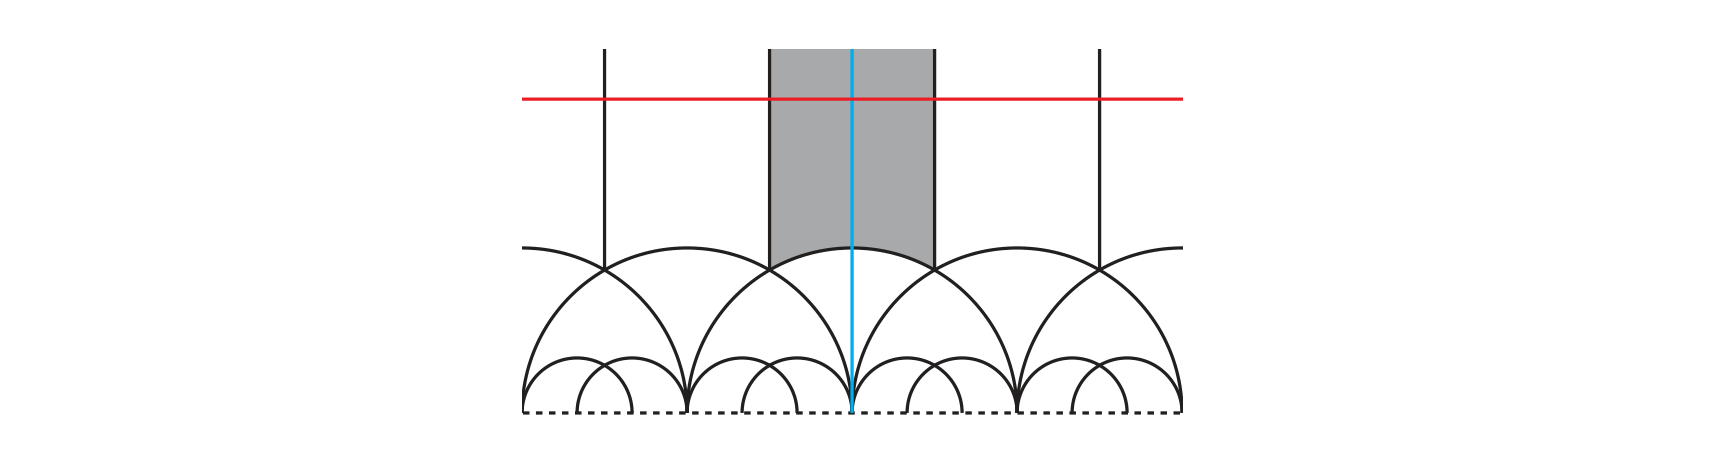
\includegraphics[width=0.6\textwidth]{figure17-1.png}
  \caption{$\mathrm{SL}_2(\Z)$ 作用在 $\mathbb H$ 上的基本域（灰色区域）。
  可以通过对模形式积分（例如沿红线或蓝线）来定义“周期”。
  （原文 p.~293，Figure 17.1）}
  \label{fig:17-1}
\end{figure}

\begin{srcex}{118}
若 $M^{\vee}=T^*X^{\vee}$，则
\begin{equation}\tag{17.96}\label{eq:17.96}
\Loc^{X^{\vee}}_{G^{\vee}}
=\bigl\{\rho\ \text{以及相伴 $X^{\vee}$-丛的平坦截面}\bigr\}.
\end{equation}
有映射
\begin{equation}\tag{17.97}\label{eq:17.97}
\pi\colon\Loc^{X^{\vee}}_{G^{\vee}}\to\Loc_{G^{\vee}},
\end{equation}
于是
\begin{equation}\tag{17.98}\label{eq:17.98}
\cL:=\pi_*\omega.
\end{equation}
我们用 $\omega$ 而不是 $\cO$，原因与我们用 $\IndCoh$ 而不是 $\QC$ 相同。
\end{srcex}

% [Tutor Note: Remark 122 的 “$P_3$-variety” 原文如此（p.291），含义并不标准：按上下文，
%  应是把 $M^{\vee}$ 的 3-移位 Poisson 结构（$P_3$）量子化为 $E_3$-代数；
%  “取上同调”指忘记 $E_3$ 结构只保留交换代数。另 (17.98) 中的 $\omega$ 是 $T^*X^{\vee}$
%  上的全纯体积形式/Canonical bundle 的平方根型对象，之所以用 $\IndCoh$ 是因为
%  $T^*X^{\vee}$ 上自然出现的是（移位）相干层而不是拟凝聚层。]

\section{自守形式的周期（A-侧）}

\begin{sectionkey}
本节从经典数论角度解释 A-侧的边界条件如何产生自守形式的周期：对子群 $H\subset G$ 积分得到
$H$-周期（Eisenstein 周期、Whittaker 周期、Hecke 周期都是特例）；更一般地，球簇 $X$
的周期理论应当由哈密顿 $G$-空间 $M=T^*X$ 的“自守量子化”来理解。
\end{sectionkey}

这种哈密顿辛几何如何从自守侧产生？我们想从经典数论的视角来呈现。

$L$-函数理论中的一个基本问题是：我们怎么知道它可以解析延拓？这在 Galois 侧不是我们能直接
触及的东西。我们谈过一点自守形式的 $L$-函数。把 $L$-函数附着到自守形式有一个直接的想法。
想法是：若 $f$ 是自守形式，则它在除有限多个位之外都非分歧。于是对所有 $p\notin S$ 有 Satake 参数。
这只意味着 Hecke 本征值。Satake 对应的全部要点是：Hecke 本征值对应于
$[F]\in G^{\vee}/G^{\vee}$。对偶群正来源于此。于是我们知道如何附着 $L$-因子：
对 $V\in\Rep(G^{\vee})$ 可以定义
\begin{equation}\tag{17.99}\label{eq:17.99}
L(f,V,s)=\sideset{}{'}\prod_{p\notin S}\frac{1}{\det(1-p^{-s}F_p)}.
\end{equation}

让我们以不同的方式再问这个问题：自守形式上的自然泛函是什么？这是问题“$\mathcal A_G$ 的边界条件
是什么”的特例。要点是：一个边界条件当然会给出 $\mathcal A_G(C)$ 上的泛函，
而 $\mathcal A_G(C)$ 是自守形式空间。让我们转到模形式的图景，故 $G=\mathrm{PSL}_2(\Z)$。
给定特定的闭链，我们可以对模形式积分得到一个数。见图 \ref{fig:17-1}。红线是 horocycle，
将给出 Eisenstein 周期。蓝线将给出 Hecke 周期。$\mathrm{SL}_2\Z$ 上任一模形式 $\varphi$
都有 $q$-展开：
\begin{equation}\tag{17.100}\label{eq:17.100}
\varphi=\sum a_n q^n,
\end{equation}
即它在 $\infty$ 处的 Laurent 展开。于是可以把 $\varphi$ 送到数
\begin{equation}\tag{17.101}\label{eq:17.101}
a_0=\int_{\text{horocycle}}\varphi\,dt.
\end{equation}
这称为 \term{Eisenstein 周期}{Eisenstein period}。（它告诉尖形式与 Eisenstein 级数之间的差别。）
可以把 $y=1$ 写成轨道
\begin{equation}\tag{17.102}\label{eq:17.102}
\int_{y=1}\varphi\,dt=\int_{N(\Z)\backslash N(\R)}\varphi\,dt,
\end{equation}
故这也称为 $N$-周期，其中
\begin{equation}\tag{17.103}\label{eq:17.103}
N=\begin{pmatrix}1&*\\&1\end{pmatrix}.
\end{equation}
系数 $a_1$ 是 Whittaker 周期。

另一个例子，沿蓝线积分，给出 Hecke 周期。即沿虚轴积分：
\begin{equation}\tag{17.104}\label{eq:17.104}
\int_0^{\infty}\varphi(iy)\,\frac{dy}{y}\,y^s.
\end{equation}
可以把它改写为
\begin{equation}\tag{17.105}\label{eq:17.105}
\int_0^{\infty}\varphi(iy)\,\frac{dy}{y}\,y^s=\sum\frac{a_n}{n^s},
\end{equation}
其中 $a_n$ 是 $\varphi$ 的 $q$-展开系数。这是 $\varphi$ 的 $L$-函数：
\begin{equation}\tag{17.106}\label{eq:17.106}
\int_0^{\infty}\varphi(iy)\,\frac{dy}{y}\,y^s
=\sum\frac{a_n}{n^s}=\frac{\Gamma(s)}{(2\pi)^s}L(\varphi,s).
\end{equation}
可以写出
\begin{equation}\tag{17.107}\label{eq:17.107}
L(\varphi,s)=\prod_p\frac{1}{1-a_p p^{-s}+p^{k-1-2s}}.
\end{equation}
当 $\varphi$ 是本征形式时，这恰好是 Hecke 本征值给出的局部 $L$-因子之积。
因子 $\Gamma(s)/(2\pi)^s$ 是 $\infty$ 处的 $L$-因子。

现在我们可能想知道：这与 Galois 侧如何相关？我们怎么知道要做这个积分？定义这个积分需要什么数据？
它与另一侧所需的数据如何相关？更抽象地定义这些周期的方式是：给定子群 $H\subset G$，
可以如下计算 $H$-周期。回忆我们有与 $G$ 相伴的局部对称空间，它是 $\Bun_G$ 的版本：
\begin{equation}\tag{17.108}\label{eq:17.108}
[G]_F=G(F)\backslash G(\mathbb A)/\text{level}.
\end{equation}
在其内部有
\begin{equation}\tag{17.109}\label{eq:17.109}
[H]_F=H(F)\backslash H(\mathbb A)/.
\end{equation}
然后可以定义 $H$-周期为
\begin{equation}\tag{17.110}\label{eq:17.110}
\mathcal{P}_H(\varphi)=\int_{H(F)\backslash H(\mathbb A)}\varphi.
\end{equation}
Eisenstein 周期来自 $H=N\subset\mathrm{PSL}_2$，Hecke 周期来自 $H=T\subset\mathrm{PSL}_2$。

\begin{srcrem}{123}
实际上我们只需要球子群 $H$。这是一个有限性条件，它给出良好的解析性质。
\end{srcrem}

% [Tutor Note: (17.109) 末尾的 “$/\,$” 在原文（p.294）中分母留空，应为与 (17.108) 中
%  “level” 相匹配的级结构（对 $H$ 取同一个 level 的子群）。作者显然省略了它。
%  另 (17.101) 的 horocycle 是 $N(\Z)\backslash N(\R)$（即 $y=1$ 的轨道），其积分给出
%  $q$-展开的常数项 $a_0$；而 $a_1$ 是 Whittaker 周期，对应 $N$-周期取非平凡特征。
%  (17.106) 的推导需要 $\varphi$ 是模形式，且 $a_n$ 按 $q=e^{2\pi i z}$ 展开。]

这来自 Terry Tao 的一篇博客文章。考虑阿贝尔 $L$-函数，即 $G=\mathrm{GL}_1=G^{\vee}$ 的
$L$-函数。例如 Riemann 与 Dedekind $\zeta$-函数是阿贝尔 $L$-函数。还有经典的 Dirichlet
$L$-函数，以及 Hecke 的推广。它们对应于 $\Gal(\overline F/F)$ 的特征。由类域论我们知道，
它们对应于 idèle 类群的特征 $\chi$：
\begin{equation}\tag{17.111}\label{eq:17.111}
\mathrm{GL}_1(F)\backslash\mathrm{GL}_1(\mathbb A).
\end{equation}
这些有时称为 \term{Hecke 本征特征}{Hecke grössencharacters}。

Riemann 把 $\zeta$-函数写成了积分。特别地，$\Xi$ 函数
\begin{equation}\tag{17.112}\label{eq:17.112}
\Xi(s)=\frac{\Gamma(s/2)}{\pi^{s/2}}\xi(s),
\end{equation}
其中可把前因子看作 $\infty$ 处的局部因子，可以写成
\begin{equation}\tag{17.113}\label{eq:17.113}
\Xi(s)=\int_0^{\infty}y^{s/2}\sum_{n=1}^{\infty}e^{-n^2\pi y}\,dy.
\end{equation}
即这是 $\theta$-函数的 Mellin 变换。

局部地（固定有限素数 $p$），在位 $v=p$ 有（局部类域论）
\begin{equation}\tag{17.114}\label{eq:17.114}
K_v^{\times}/\cO_v^{\times}\simeq\Z.
\end{equation}
例如 $\Q_p^{\times}/\Z_p^{\times}\simeq\Z$。在其中我们有
$\varpi\in K_v^{\times}/\cO_v^{\times}$，它对应 $1\in\Z$，即
$p\in\Q_p^{\times}/\Z_p^{\times}$。考虑非分歧局部特征
\begin{equation}\tag{17.115}\label{eq:17.115}
\chi_v\colon K_v^{\times}/\cO_v^{\times}\to\C^{\times}.
\end{equation}
它由单个数确定，即 $\chi_v\in\C^{\times}$。这对应于 $F_v$ 以 $\chi_v$ 作用的
一维 Galois 表示。关键观察：这个特征在 $0$ 处的 $L$-值是
\begin{equation}\tag{17.116}\label{eq:17.116}
L(\chi_v,0)=\frac{1}{1-\chi_v}
=\operatorname{Tr}(\chi_v,\operatorname{Sym}^{\bullet}\C)
=\sum_{n\ge 0}\chi_v^n.
\end{equation}
要点是我们可以把它改写为 $K^{\times}/\cO^{\times}$ 上的积分。特别地可以写
\begin{align}
L(\chi_v,0)&=\frac{1}{1-\chi_v}
=\operatorname{Tr}(\chi_v,\operatorname{Sym}^{\bullet}\C)\tag{17.117}\label{eq:17.117}\\
&=\sum_{n\ge 0}\chi_v^n\tag{17.118}\label{eq:17.118}\\
&=\sum_{n=0}^{\infty}\chi_v\bigl(\varpi^n\in K^{\times}/\cO^{\times}\bigr)\tag{17.119}\label{eq:17.119}\\
&=\int_{K_v^{\times}}\chi_v(x)\cdot1_{\cO_v}\,d^*x.\tag{17.120}\label{eq:17.120}
\end{align}
关键观察是，这个特征函数是\term{局部基本函数}{local basic function}：
\begin{equation}\tag{17.121}\label{eq:17.121}
\Phi_v=1_{\cO_v}.
\end{equation}
$L$-因子可以写成
\begin{equation}\tag{17.122}\label{eq:17.122}
L_v(\chi_v,s)=\int_{K_v^{\times}}\chi_v\Phi_v(x)\,d^*x\cdot|x|_v^s.
\end{equation}
这是 $\Phi_v=1_{\cO}$ 的 Mellin 变换。

让我们退一步。我们在做 $\mathbb G_m\curvearrowright\mathbb A^1$ 的 Fourier 理论。
想 $\mathbb A^1\simeq K\simeq\Q_p$。在其中 $1_{\Z_p}=1_{\cO}$，我们想按
$\mathbb G_m$-作用分解它。$\Phi_v=1_{\cO_v}=1_{\Z_p\subset\Q_p}$ 的实版本是 Gaussian：
\begin{equation}\tag{17.123}\label{eq:17.123}
\Phi_{\infty}(x)=e^{-\pi x^2},
\end{equation}
而 $\infty$ 处的局部 $L$-因子是
\begin{equation}\tag{17.124}\label{eq:17.124}
L_{\infty}=\int_{\R^{\times}}\Phi_{\infty}(x)e^{-\pi x^2}.
\end{equation}

\subsection{Iwasawa--Tate}

\begin{sectionkey}
本小节把特征 $\chi$ 的 $L$-函数写成阿黛尔空间上的积分（Iwasawa--Tate 公式）：
它是对 $\theta$-级数求和后用 $\chi$ 配对，本质上是 $K^\times/\cO^\times\simeq\Z$ 上的
Fourier/Pontrjagin 对偶；在函数域情形这给出几何版本的 $\Theta=\pi_*1$。
\end{sectionkey}

可以把特征的 $L$-函数改写为
\begin{equation}\tag{17.125}\label{eq:17.125}
L(\chi,s)=\int_{F^{\times}\backslash\mathrm{GL}_1(\mathbb A)}
\chi(x)\cdot\sum_{\gamma\in F}\Phi(\gamma x)\,d^*x,
\end{equation}
其中
\begin{equation}\tag{17.126}\label{eq:17.126}
\Phi=\prod_v\Phi_v.
\end{equation}
这是
\begin{equation}\tag{17.127}\label{eq:17.127}
\sideset{}{'}\prod_{F_v}\mathbb A^1_{F_v}
\end{equation}
上的函数。这是对（比如）$\Q$ 的求和，那么它与之前对 $\Z$ 的求和如何相关？嗯：
\begin{equation}\tag{17.128}\label{eq:17.128}
\sum_{\gamma\in F}\Phi(\gamma\cdot x)=\sum_{\gamma\in\cO_F}\Phi_{\infty}(\gamma x),
\end{equation}
即我们得到 $x$ 的平移上的 Gaussian 之和。这就是 $\theta$-级数。有算子
\begin{equation}\tag{17.129}\label{eq:17.129}
\Theta\colon\operatorname{Fun}\bigl(\mathbb A^1_{\mathbb A}\bigr)
\to\operatorname{Fun}\bigl([\mathrm{GL}_1]\bigr),
\end{equation}
它由对所有平移求和给出：
\begin{equation}\tag{17.130}\label{eq:17.130}
\Theta(\Phi)=\sum_{\gamma\in F}\Phi(\gamma\cdot x).
\end{equation}
注意 $\Phi\in\operatorname{Fun}(\mathbb A^1_{\mathbb A})$，事实上
\begin{equation}\tag{17.131}\label{eq:17.131}
L(\chi)=\int\chi\Theta(\Phi)=\langle\chi,\Theta\rangle.
\end{equation}

在函数域情形我们有
\begin{equation}\tag{17.132}\label{eq:17.132}
\operatorname{Pic}(C)(k)=F^{\times}\backslash\mathbb A^{\times}\big/\mathbb A_A^{\times}.
\end{equation}
则
\begin{equation}\tag{17.133}\label{eq:17.133}
\Theta_{\Phi}\colon\operatorname{Pic}\ni L\mapsto
\sum_{\gamma\in F^{\times}}\Phi(\gamma\cdot L)=\# H^0(C,L).
\end{equation}
几何地，
\begin{equation}\tag{17.134}\label{eq:17.134}
\begin{array}{ccc}
\operatorname{Pic}^{\mathbb A^1} & = & \text{线丛及相伴 $\mathbb A^1$-丛的截面}\\[2pt]
\downarrow{\scriptstyle \pi} & & \\[2pt]
\operatorname{Pic} & = & \text{线丛}
\end{array}
\end{equation}
且
\begin{equation}\tag{17.135}\label{eq:17.135}
\Theta=\pi_*1.
\end{equation}
现在我们可以非常容易地把它推广到非阿贝尔群。

% [Tutor Note: (17.116)--(17.120) 的关键是把 $\Z$ 上的几何级数 $\sum\chi_v^n$ 写成
%  $K_v^\times$ 上的积分：$\varpi^n$ 对应 $n\in\Z$，而 $1_{\cO_v}$ 是“基本函数”。
%  这正是 Iwasawa--Tate 理论的核心：$L$-因子是局部基本函数的 Mellin 变换。
%  (17.128) 中求和从 $\gamma\in F$ 换成 $\gamma\in\cO_F$，原因是 $\Phi_\infty$ 为 Gaussian
%  而其余 $\Phi_v=1_{\cO_v}$ 只在整点上非零（对 $F=\Q$ 时 $\cO_F=\Z$）；这一步是
%  Poisson 求和/函数方程的技术核心，作者未展开。]

\section{一般版本}

\begin{sectionkey}
本节把周期理论推广到任意球簇 $G\curvearrowright X$：周期 $P_X$ 由 $\Bun^X_G\to\Bun_G$
的推出给出，而对偶侧由哈密顿 $G^{\vee}$-空间 $M^{\vee}$ 与 Plancherel 测度刻画；
由此陈述三个猜想（整体数值、整体几何、局部几何），把周期与 $L$-函数、Plancherel 测度与
$\Shv(X(K)/G(\cO))$ 的 Satake 对应联系起来。
\end{sectionkey}

起点数据是群作用在簇上：$G\curvearrowright X$。

\begin{srcex}{119}
取 $G\curvearrowright G/H$、$\mathrm{PSL}_2\curvearrowright\mathrm{PSL}_2/T$ 以及
$\mathrm{GL}_1\curvearrowright\mathbb A^1$，就还原到我们之前考虑的具体情形。
\end{srcex}

现在我们有
\begin{equation}\tag{17.136}\label{eq:17.136}
\sideset{}{'}\prod X(K)/G(\cO)=\Bun^X_G=\operatorname{Map}(C,X/G),
\end{equation}
它由带 $X$-丛截面的 $G$-丛组成。有投影映射
\begin{equation}\tag{17.137}\label{eq:17.137}
\begin{array}{ccc}
\sideset{}{'}\prod X(K)/G(\cO) & \Bun^X_G & \operatorname{Map}(C,X/G)\\[2pt]
\downarrow{\scriptstyle\pi} & \downarrow{\scriptstyle\pi}
& \downarrow{\scriptstyle\pi}\\[2pt]
G(F)\backslash G(\mathbb A)/G(\cO_{\mathbb A}) & \Bun_G
& \operatorname{Map}(C,\mathrm{pt}/G)
\end{array}
\end{equation}

\begin{srcex}{120}
若 $X=G/H$，则 $\Bun^X_G=\Bun_H$。
\end{srcex}

于是现在有自然映射。自守形式的 $X$-周期就是
\begin{equation}\tag{17.138}\label{eq:17.138}
\mathcal{P}_X(\varphi)=\langle\Theta_X,\varphi\rangle_{\Bun_G},
\end{equation}
其中
\begin{equation}\tag{17.139}\label{eq:17.139}
\Theta_X=\pi_*1.
\end{equation}
或者由伴随可以写
\begin{equation}\tag{17.140}\label{eq:17.140}
\mathcal{P}_X(\varphi)=\langle\Theta_X,\varphi\rangle_{\Bun_G}
=\int_{\Bun^X_G}\pi^*\varphi.
\end{equation}

我们在忽略这些积分与求和的收敛性问题。需要知道一些解析性质，它们将来自对 $X$ 的强有限性假设。
这就是球簇理论登场之处。

Ben-Zvi--Sakellaridis--Venkatesh 即将开展的工作的要点如下。设 $G\curvearrowright X$ 是球性的。
这定义了自守理论 $\mathcal A_G$ 的边界条件。要点是：周期理论是边界数据理论的三维部分。
但从物理上说，我们应该使用哈密顿 $G$-空间，而不只是 $G$-空间。由 $G\curvearrowright X$ 的数据，
得到哈密顿 $G$-空间 $M=T^*X\circlearrowleft G$。断言是：周期理论是\term{微局部}{microlocal}的。
即它真正是关于 $M$（而不是 $X$）的“自守量子化”。在 Tate 的论文中，关键要素是函数方程来自
在 $\mathbb A^1$ 上做 Fourier 变换。但 Fourier 变换不是 $\mathbb A^1$ 的对称性，而是
$T^*\mathbb A^1$ 由 90 度旋转给出的对称性。$L$-函数不依赖 $\mathbb A^1$ 而依赖
$T^*\mathbb A^1$ 这一事实，意味着它在此对称性下不变，从而特别地在 Fourier 变换下不变，
这就给出函数方程。

事实上有很多与 $G\curvearrowright M$ 相伴的周期例子，其中 $M$ 不是余切丛。例如 Whittaker
周期 $a_1$ 自然地来自一个\term{扭余切丛}{twisted cotangent bundle}。还有所谓
\term{theta 对应}{theta correspondence}，它来自研究不是余切丛的辛空间。这些一般来自一般辛表示
$G\curvearrowright V$，它可能不是 $W\oplus W^*$。故这是周期的一个重要来源。

\begin{srcrem}{124}
如上所述，使所有这些积分收敛所需的有限性来自 $X$ 是球性的。对 $M$ 的类似条件是什么？
我们坚持要求 $\cO(M)^G$ 是 Poisson 交换的。这些称为\term{重数 1 哈密顿空间}{multiplicity 1
Hamiltonian space}。超球性（hyperspherical）则是此条件再加几条额外条件。
\end{srcrem}

这个名字的动机来自 hypertoric 簇。这个名字来自它们是超 Kähler 的。

% [Tutor Note: Remark 124 的末两句在原文（p.297）中指代混乱：“The name is motivated by
%  hypertoric varieties. This name comes from them being hyperkähler.”——两个 “name” 指的
%  应是不同的东西（“multiplicity 1” 的命名动机与 “hypertoric” 的词源）。按数学含义，
%  hypertoric 簇是“超 Kähler 的环面簇”，其名称来自 hyperkähler + toric；
%  而“重数 1”指的是 $\cO(M)^G$ 在 Poisson 交换意义下的重数。这里照原文译出并提示。]

BZ-Sakellaridis-Venkatesh 的想法是用边界条件理论来组织周期理论。于是自守侧的周期在 B-侧
将有对偶。这有点模糊，但由此我们可以用重构提取对偶群的哈密顿簇：
\begin{equation}\tag{17.141}\label{eq:17.141}
G^{\vee}\curvearrowright M^{\vee}.
\end{equation}
我们说过 $G^{\vee}\curvearrowright M^{\vee}$ 与 $L$-函数相关，而 $G\curvearrowright M$
与周期相关。故这建立了周期与 $L$-函数之间的桥梁。

\begin{srcconj}{3}（整体数值/算术）
自守形式的 $X$-周期的范数由相应的 $L$-函数给出：
\begin{equation}\tag{17.142}\label{eq:17.142}
|\mathcal{P}_X(\varphi)|^2=L(\rho,M^{\vee}),
\end{equation}
其中 $\varphi$ 对应于 $\rho\colon\Gal\to G^{\vee}$。
\end{srcconj}

\begin{srcrem}{125}
这里 $|\cdot|^2$ 来自如下事实：这秘密地是关于 $M=T^*X$ 而不只是 $X$ 的。
\end{srcrem}

现在可以到处跑并做出大量猜想。

\begin{srcconj}{4}（整体几何）
回忆我们有
\begin{equation}\tag{17.143}\label{eq:17.143}
\cL_{M^{\vee}}\in\QC^{!}\bigl(\Loc_{G^{\vee}}\bigr)=\mathcal B_{G^{\vee}}(C),
\end{equation}
由沿
\begin{equation}\tag{17.144}\label{eq:17.144}
\Loc^{X^{\vee}}_{G^{\vee}}\to\Loc_{G^{\vee}}
\end{equation}
的前推给出。我们可以在 A-侧做同样的事情。我们有
\begin{equation}\tag{17.145}\label{eq:17.145}
\mathcal A_G(C)=\Shv\bigl(\Bun_G(C)\bigr).
\end{equation}
在其内部得到周期层，即
\begin{equation}\tag{17.146}\label{eq:17.146}
\mathcal{P}_X=\pi_*k,
\end{equation}
其中
\begin{equation}\tag{17.147}\label{eq:17.147}
\pi\colon\Bun^X_G\to\Bun_G.
\end{equation}
\end{srcconj}

$M^{\vee}$ 从自守形式的观点看是什么意思？在自守侧，Sakellaridis--Venkatesh 写了 [SV17]，
其中研究整体周期理论与表示论（调和分析）中局部问题之间的关系。

对局部域上的 $G$-簇该做什么？首先考虑局部算术情形。于是可以考虑 $X$ 在 $K$ 上的函数空间
$X(K)$。群 $G(K)$ 作用在其上，故可以（比如）把 $L^2(X(K))$ 分解为 $G(K)$ 的表示。
这正是局部 Langlands 对应中出现的那类对象。

不那么贪心的做法是看球函数的概念。这意味着考虑 $X(K)$ 上在 $G(\cO)$ 的正半部分下不变的函数。
这现在是 Hecke 代数的一个表示：
\begin{equation}\tag{17.148}\label{eq:17.148}
X(K)/X(\cO)\curvearrowright k\bigl[G(\cO)\backslash G(K)/G(\cO)\bigr]
\simeq\bigl|\Rep(G^{\vee})\bigr|.
\end{equation}
% [Tutor Note: 原文 p.298 的 "the positive half of $G(\cO)$" 一语，作者在本书中未另作定义；
%  按 (17.149) 的语境，它指 $G(\cO)$ 里相对 Iwahori 子群的正向部分，"在该部分下不变"
%  应读作相应的 Iwahori 不变条件，而与 "$G(\cO)$ 本身分正负半" 无关。
%  [译者按（无外部依据）：仅据 (17.149) 上下文与 Iwahori 分解的通行约定读出。]]
$X$ 是球簇，等价于 $G(\cO)\curvearrowright X(K)$ 有离散轨道。例如仿射 Grassmann 簇。

于是现在考虑 Hecke 代数作用在球函数上：
\begin{equation}\tag{17.149}\label{eq:17.149}
\cH\simeq\bigl|\Rep(G^{\vee})\bigr|\curvearrowright L^2\bigl(X(K)/G(\cO)\bigr).
\end{equation}
$\Phi=1_{X(\cO)}$ 是球函数。$\Theta$ 算子是
\begin{equation}\tag{17.150}\label{eq:17.150}
\Theta\colon\sideset{}{'}\bigotimes L^2\bigl(X(K)/G(\cO)\bigr)\to L^2(\Bun_G),
\end{equation}
且
\begin{equation}\tag{17.151}\label{eq:17.151}
\Theta(\Phi)=\mathcal{P}_X.
\end{equation}

% [Tutor Note: (17.148) 左端的 $X(K)/X(\cO)$ 在原文（p.298）中如此印出，但按上下文
%  （球函数是 $X(K)$ 上 $G(\cO)$-不变的函数）这里应为 $X(K)/G(\cO)$，即
%  “$G(\cO)$ 作用在 $X(K)$ 上”。分母写成 $X(\cO)$ 是原文笔误（也可能是把
%  商 $X(K)/G(\cO)$ 与 $X(\cO)$ 的记号混用）。这里照原文保留并在 (17.148) 中提示；
%  (17.149) 起即改用正确的 $X(K)/G(\cO)$。]

所以我们想理解 $L^2(X(K))$ 的 Plancherel 测度。这是 $G(K)$ 的酉表示集合上的测度。
由局部 Langlands 对应，它与局部 Langlands 参数相匹配。代替它，我们可以考虑球函数并尝试按
$\cH$-作用分解。回忆
\begin{equation}\tag{17.152}\label{eq:17.152}
\cH\simeq\bigl|\Rep(G^{\vee})\bigr|\simeq\cO\bigl(G^{\vee}/G^{\vee}\bigr).
\end{equation}

我们甚至不会尝试分解整个空间。只看这个基本函数 $\Phi$。

所以我们问的是调和分析问题，而我们将几何地回答它。给定 Hilbert 空间中的一个状态 $\Phi$，
从中得到的是算子代数谱上的一个谱测度。在我们的情形，我们编码包含 $\Phi$ 的 $\cH$-作用的
轨道的所有不同乘积，即
\begin{equation}\tag{17.153}\label{eq:17.153}
\langle H_v\cdot\Phi,H_w\cdot\Phi\rangle
\end{equation}
其中 $H_v,H_w\in\cH\simeq|\Rep(G^{\vee})|$。这决定了 Hecke 代数谱上的测度，
即 Plancherel 测度。这告诉我们 $\Phi$ 如何分解，因为 $\cH\simeq|\Rep(G^{\vee})|$。
事实上，同一个表示控制了 $X$-周期理论中出现的整体 $L$-函数。“（对 $X$ 的）周期的平方”
看起来就像 $X$ 的 Plancherel 测度的 Euler 积。

如何几何地思考这一点？这将解释对偶边界条件从何而来。要点是
$M^{\vee}\circlearrowleft G^{\vee}$ 是 $X(K)/G(\cO)$ 的 Plancherel 测度的范畴化形式。

同一个问题的几何版本如下。我们用层替换函数：
\begin{equation}\tag{17.154}\label{eq:17.154}
\Shv\bigl(X(K)/G(\cO)\bigr).
\end{equation}

\begin{srcex}{121}
若 $X=G$ 且 $G\times G\curvearrowright G$，则这还原仿射 Grassmann 簇
$G(\cO)\backslash G(K)/G(\cO)$。
\end{srcex}

球性条件模仿了这个例子的离散方面。在其中有一个基本层：
\begin{equation}\tag{17.155}\label{eq:17.155}
\Phi=k_{X(\cO)}\in\Shv\bigl(X(K)/G(\cO)\bigr).
\end{equation}
即我们用常值层替换特征函数。

那 Plancherel 测度呢？可以几何地做同样的事情。用 $\Hom$ 替换配对，于是考虑
\begin{equation}\tag{17.156}\label{eq:17.156}
\Hom_{\Shv}\bigl(H_V*\Phi,H_W*\Phi\bigr).
\end{equation}
这个空间上的 Frobenius 迹将给我们经典调和分析。这一切都由单个对象捕获，
即 Plancherel 测度的类似物：它由
\begin{equation}\tag{17.157}\label{eq:17.157}
\cA_X=\End_{\cH}(\Phi)
\end{equation}
捕获，这里是内 Hom，即有函子
\begin{equation}\tag{17.158}\label{eq:17.158}
\cH\to\Shv\bigl(X(K)/G(\cO)\bigr),
\end{equation}
由作用在 $\Phi$ 上给出。有一个伴随，由 $\Hom(\Phi,-)$ 给出。即 $\cA$ 是
\begin{equation}\tag{17.159}\label{eq:17.159}
\cH=\Shv\bigl(G(\cO)\backslash G(K)/G(\cO)\bigr)=\mathcal A_G(S^2)
\end{equation}
中的代数对象。

它不只是某个旧代数对象，事实上它是结合的因子化代数。即它是
$\mathcal A_G(S^2)$ 中 $E_3$-代数对象的某种版本。但这正是我们出发时的数据：
从边界条件出发，我们（除其他东西外）找到了线算子中的一个代数。当我们仔细思考在局部情形
得到什么时，$\cA_X$ 恰好是边界条件上局部算子的代数。于是对偶哈密顿空间是
\begin{equation}\tag{17.160}\label{eq:17.160}
M^{\vee}=\Spec_{/(\mathfrak g^{\vee*}/G^{\vee})}(\cA_X)
\in\mathcal A_G(S^2),
\end{equation}
并回忆
\begin{equation}\tag{17.161}\label{eq:17.161}
\mathcal A_G(S^2)=\mathcal B_{G^{\vee}}(S^2)
=\QC\bigl(\mathfrak g^{\vee*}/G^{\vee}\bigr),
\end{equation}
即 $M^{\vee}$ 是 Plancherel 测度支撑的几何版本。矩映射的支撑就是 Plancherel 测度的支撑。

Sakellaridis、Sakellaridis--Venkatesh 以及 Sakellaridis--Wang 计算了大量关于 Plancherel
测度的内容（原文此处标注 cite$^3$）。于是我们可以精确描述 $M^{\vee}$。然后可以陈述一些猜想。
其中最基本的一条如下。

\begin{srcconj}{5}（局部几何）
边界上的线算子相匹配：
\begin{equation}\tag{17.162}\label{eq:17.162}
\Shv\bigl(X(K)/G(\cO)\bigr)\simeq\QC\bigl(M^{\vee}/G^{\vee}\bigr),
\end{equation}
且与如下作用相容：
\begin{equation}\tag{17.163}\label{eq:17.163}
\cH\simeq\QC\bigl(\mathfrak g^{\vee*}/G^{\vee}\bigr).
\end{equation}
（注：后一个同构是 Satake。）
\end{srcconj}

% [Tutor Note: (17.148) 与 (17.152) 中的 $|\Rep(G^{\vee})|$ 记号并不标准：作者用它表示
%  “Hecke 代数所对应的范畴/代数”，即 Satake 等价 $k[G(\cO)\backslash G(K)/G(\cO)]
%  \simeq\Rep(G^{\vee})$ 的（导出）版本；竖线可能表示取“底层范畴”或“同伦范畴”。
%  阅读时把它当作 Satake 等价的简写即可。(17.159)--(17.161) 则说明：边界条件的线算子范畴
%  $\mathcal A_G(S^2)$ 同构于 $\QC(\mathfrak g^{\vee*}/G^{\vee})$，而 $M^{\vee}$ 相对谱
%  正是 Plancherel 测度支撑的几何化；(17.162) 把 Plancherel 测度的支撑与
%  $\Shv(X(K)/G(\cO))$ 的谱联系起来。最后，Conjecture 3、4、5 分别对应数值（周期范数）、
%  整体几何（$L$-层与周期层）、局部几何（Plancherel 测度）三个层次。]
